
This section describes some of the main aspects of the software development
process and software lifecycle as specified in CENELEC EN 50128

\subsection{Objectives}
\label{sec:objectives}

The two most important goals of the SW development lifecycle model of CENELEC EN
50128 standard are the separation of the lifecycle into well-defined phases and
the focus on the production and recording of all documentation of the
development process. To achieve this, an appropriate software lifecycle model
must be used and appropriate roles and responsibilities must be assigned. For
this, the standard specifies several constrains which must be fulfilled.

\subsection{Organisational Structure and Roles}
\label{sec:organ-struct-roles}

CENELEC EN 50128 defines a set of required roles for the development of SIL4 (or
SIL3) compliant software. Theses roles are specified in 5.1.2.10 of the
standard. This distribution and in particular the required separation of several
of the roles is mandatory for the development process.

\begin{figure}[ht]
  \centering
  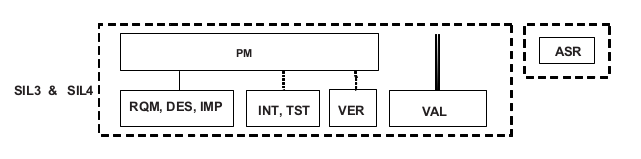
\includegraphics[width=\textwidth]{CenelecRoles}
  \caption{Preferred Organisational Roles~\cite{EN-50128}}
  \label{fig:preferred-roles}
\end{figure}

Figure~\ref{fig:preferred-roles} shows the preferred organisational structure
according to CENELEC EN 50128, in particular the role separations, e.g., the
verifier (VER) cannot be the same person as tester, the requirements manager
(RQM) must be a different person than the integrator (INT) and the validator
(VAL) must be independent of the project manager (PM) in the sense that the VAL
does not report to the RQM.

\subsection{Documentation}
\label{sec:documentation}

The development according to CENELEC EN 50128 is document-centered and many
mandatory documents mus be created.  In such a development process, not only the
SW shall be of concern, but also the generated documentation, in particular the
update of existing documentation and the verification of consistency regarding
related or referenced documents.

\subsubsection{Consistency of Documentation}
\label{sec:cons-docum}

It is mandatory to have a consistent definition and usage of all terms,
abbreviations etc. in all produced documents. This is especially important if
the development process uses small scale iterations, as the consistency must be
assured and restored if necessary after each iteration. In particular, it must
be assured at all times, that dependent documents, i.e., in hierarchical
relation do not contradict each other.

\subsubsection{Traceability of Requirements}
\label{sec:trac-requ}

For each of the generated documents, the traceability must be assured by
referencing all other concerned documents, by specifying unique reference
numbers and by versioning of the documents. Like consistency, traceability is a
mandatory aspect which is often not a concern in more general software
development processes.

\subsection{Support Tool Usage}
\label{sec:tool-usage}

Tools to support the development process are classified into three different
classes: T1 for tools which generate no output which can have any direct or
indirect effect on the resulting code, T2 for tools which support test or
verification of designs or executable code where the tool may fail to indicate
errors but cannot influence the executable code, and finally T3 for tools which
may directly or indirectly influence the code or data of the SW for the safety
related system.

The selected tools shall be able to cooperate in the sense that the output of
one tool is usable as input for another tool. The usage of tools of the classes
T2 and T3 must be justified by giving evidence that erroneous can be
detected. It is possible to replace manual tasks by automatization using tools,
in this case evidence for the appropriateness of the tools must be delivered.


%%% Local Variables:
%%% mode: latex
%%% TeX-master: "wp-2.2"
%%% End:
